\documentclass{article}
\usepackage{helvet}


\usepackage{cite}
\usepackage{amsmath,amssymb,amsfonts}
\usepackage{algorithmic}
\usepackage{graphicx}
\usepackage{textcomp}
\usepackage{xcolor}
\usepackage{hyperref}
\usepackage{placeins}
\usepackage{graphicx}
\usepackage{subcaption}



\def\BibTeX{{\rm B\kern-.05em{\sc i\kern-.025em b}\kern-.08em
    T\kern-.1667em\lower.7ex\hbox{E}\kern-.125emX}}


\title{Assignment 1: CS 754, Spring 2024-25}
\author{
\IEEEauthorblockN{
    \begin{tabular}{cccc}
        \begin{minipage}[t]{0.23\textwidth}
            \centering
            Amitesh Shekhar\\
            IIT Bombay\\
            22b0014@iitb.ac.in
        \end{minipage} & 
        \begin{minipage}[t]{0.23\textwidth}
            \centering
            Anupam Rawat\\
            IIT Bombay\\
            22b3982@iitb.ac.in
        \end{minipage} & 
        \begin{minipage}[t]{0.23\textwidth}
            \centering
            Toshan Achintya Golla\\
            IIT Bombay\\
            22b2234@iitb.ac.in
        \end{minipage} \\
        \\ 
    \end{tabular}
}
}

\date{February 01, 2025}


\usepackage{amsmath}
\usepackage{amssymb}
\usepackage{hyperref}
\usepackage{ulem,graphicx}
\usepackage[margin=0.5in]{geometry}

\begin{document}
\maketitle

\\
\\

\textbf{Declaration:} The work submitted is our own, and
we have adhered to the principles of academic honesty while completing and submitting this work. We have not
referred to any unauthorized sources, and we have not used generative AI tools for the work submitted here.

\begin{enumerate}
    \item Construct a synthetic image $\boldsymbol{f}$ of size $32 \times 32$ in the form of a sparse linear combination of $k$ randomly chosen 2D DCT basis vectors. Simulate $m$ compressive measurements of this image in the form $\boldsymbol{y} = \boldsymbol{\Phi} \text{vec}(\boldsymbol{f})$ where $\text{vec}(\boldsymbol{f})$ stands for a vectorized form of $\boldsymbol{f}$, $\boldsymbol{y}$ contains $m$ elements and $\boldsymbol{\Phi}$ has size $m \times 1024$. The elements of $\boldsymbol{\Phi}$ should be independently drawn from a Rademacher matrix (i.e. the values of the entries should independently be $-1$ and $+1$ with probability $0.5$). Your job is to implement the OMP algorithm to recover $\boldsymbol{f}$ from $\boldsymbol{y}, \boldsymbol{\Phi}$ for $k \in \{5,10,20,30,50,100,150,200\}$ and $m \in \{100,200,...,1000\}$. In the OMP iterations, you may assume knowledge of the true value of $k$. Each time, you should record the value of the RMSE given by $\|\text{vec}(\boldsymbol{f}) - \text{vec}(\boldsymbol{\hat{f}})\|_2/\|\text{vec}(\boldsymbol{f})\|_2$. For $k \in \{5,50,200\}$, you should plot a graph of RMSE versus $m$ and plot the reconstructed images with appropriate captions declaring the value of $k,m$. Also plot the ground truth image. For $m \in \{500,700\}$, you should plot a graph of RMSE versus $k$ and plot the reconstructed images with appropriate captions declaring the value of $k,m$. Also plot the ground truth image. Comment on the behaviour of these plots. Repeat all these tasks with the CoSAMP, another greedy algorithm from equation (10) of the paper `CoSaMP: iterative signal recovery from incomplete and inaccurate samples' which you can find at \url{https://dl.acm.org/doi/10.1145/1859204.1859229}. For implementing this algorithm, you should again assume knowledge of the true $k$. A local copy of this paper is also uploaded onto the homework folder. \textsf{[15 + 15 = 30 points]}
\end{enumerate}
        \makebox[0pt][l]{\hspace{-7pt}\textit{Soln:}} % Aligns "Answer:" to the left
    \\
\subsection*{OMP}
\begin{figure}[h!]
    \centering
        \centering
        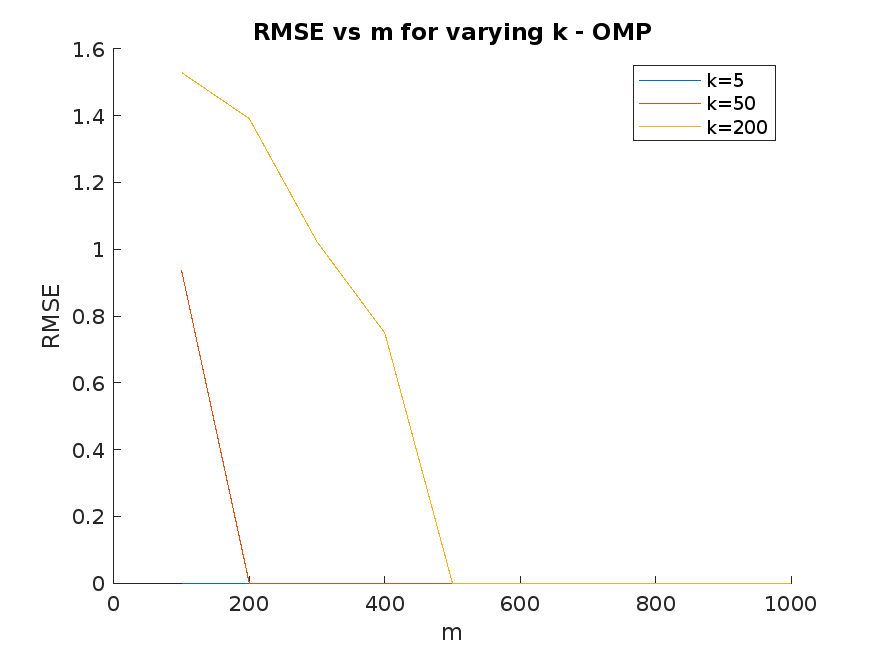
\includegraphics[width=0.5\textwidth]{HomeWork_1/5/images/OMP_k.png}
        \caption{Plot for RMSE vs m for OMP}
\end{figure}
\begin{figure}[h!]
        \centering
        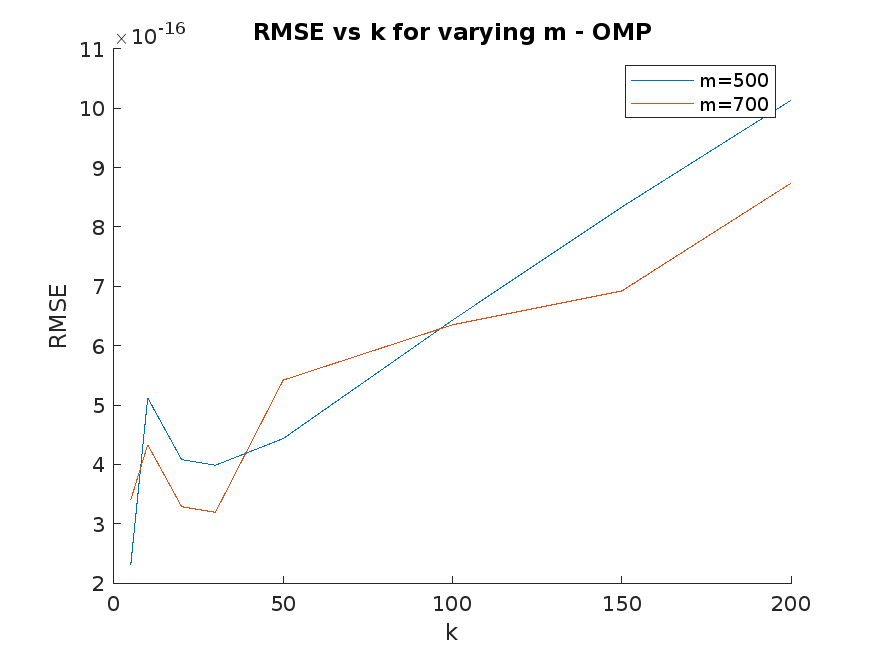
\includegraphics[width=0.5\textwidth]{HomeWork_1/5/images/OMP_m.png}
        \caption{Plot for RMSE vs k for OMP}
\end{figure}
\begin{figure}[h!]
        \centering
        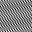
\includegraphics[width=0.25\textwidth]{HomeWork_1/5/images/orig_OMP_k=5.png}
        \caption{Original Image for k=5}
\end{figure}

\begin{figure}[h!]
    \centering
    \begin{minipage}{0.1\textwidth}
        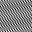
\includegraphics[width=\textwidth]{HomeWork_1/5/images/recon_p1_OMP_k=5_m=100.png}
        \caption{Reconstructed for m=100}
    \end{minipage}
    \hspace{0.5cm}
    \begin{minipage}{0.1\textwidth}
        \centering
        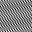
\includegraphics[width=\textwidth]{HomeWork_1/5/images/recon_p1_OMP_k=5_m=200.png}
        \caption{Reconstructed for m=200}
    \end{minipage}
    \hspace{0.5cm}
    \begin{minipage}{0.1\textwidth}
        \centering
        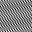
\includegraphics[width=\textwidth]{HomeWork_1/5/images/recon_p1_OMP_k=5_m=300.png}
        \caption{Reconstructed for m=300}
    \end{minipage}
    \hspace{0.5cm}
    \begin{minipage}{0.1\textwidth}
        \centering
        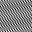
\includegraphics[width=\textwidth]{HomeWork_1/5/images/recon_p1_OMP_k=5_m=400.png}
        \caption{Reconstructed for m=400}
    \end{minipage}
    \hspace{0.5cm}
    \begin{minipage}{0.1\textwidth}
        \centering
        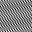
\includegraphics[width=\textwidth]{HomeWork_1/5/images/recon_p1_OMP_k=5_m=500.png}
        \caption{Reconstructed for m=500}
    \end{minipage}

    \vspace{1cm} % Add space between rows

    \begin{minipage}{0.1\textwidth}
        \centering
        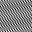
\includegraphics[width=\textwidth]{HomeWork_1/5/images/recon_p1_OMP_k=5_m=600.png}
        \caption{Reconstructed for m=600}
    \end{minipage}
    \hspace{0.5cm}
    \begin{minipage}{0.1\textwidth}
        \centering
        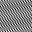
\includegraphics[width=\textwidth]{HomeWork_1/5/images/recon_p1_OMP_k=5_m=700.png}
        \caption{Reconstructed for m=700}
    \end{minipage}
    \hspace{0.5cm}
    \begin{minipage}{0.1\textwidth}
        \centering
        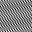
\includegraphics[width=\textwidth]{HomeWork_1/5/images/recon_p1_OMP_k=5_m=800.png}
        \caption{\small Reconstructed for m=800}
    \end{minipage}
    \hspace{0.5cm}
    \begin{minipage}{0.1\textwidth}
        \centering
        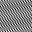
\includegraphics[width=\textwidth]{HomeWork_1/5/images/recon_p1_OMP_k=5_m=900.png}
        \caption{Reconstructed for m=900}
    \end{minipage}
    \hspace{0.5cm}
    \begin{minipage}{0.1\textwidth}
        \centering
        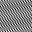
\includegraphics[width=\textwidth]{HomeWork_1/5/images/recon_p1_OMP_k=5_m=1000.png}
        \caption{Reconstructed for m=1000}
    \end{minipage}
\end{figure}

\begin{figure}[h!]
        \centering
        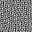
\includegraphics[width=0.25\textwidth]{HomeWork_1/5/images/orig_OMP_k=50.png}
        \caption{Original Image for k=50}
\end{figure}

\begin{figure}[h!]
    \centering
    \begin{minipage}{0.1\textwidth}
        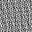
\includegraphics[width=\textwidth]{HomeWork_1/5/images/recon_p1_OMP_k=50_m=100.png}
        \caption{Reconstructed for m=100}
    \end{minipage}
    \hspace{0.5cm}
    \begin{minipage}{0.1\textwidth}
        \centering
        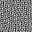
\includegraphics[width=\textwidth]{HomeWork_1/5/images/recon_p1_OMP_k=50_m=200.png}
        \caption{Reconstructed for m=200}
    \end{minipage}
    \hspace{0.5cm}
    \begin{minipage}{0.1\textwidth}
        \centering
        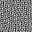
\includegraphics[width=\textwidth]{HomeWork_1/5/images/recon_p1_OMP_k=50_m=300.png}
        \caption{Reconstructed for m=300}
    \end{minipage}
    \hspace{0.5cm}
    \begin{minipage}{0.1\textwidth}
        \centering
        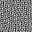
\includegraphics[width=\textwidth]{HomeWork_1/5/images/recon_p1_OMP_k=50_m=400.png}
        \caption{Reconstructed for m=400}
    \end{minipage}
    \hspace{0.5cm}
    \begin{minipage}{0.1\textwidth}
        \centering
        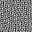
\includegraphics[width=\textwidth]{HomeWork_1/5/images/recon_p1_OMP_k=50_m=500.png}
        \caption{Reconstructed for m=500}
    \end{minipage}

    \vspace{1cm} % Add space between rows

    \begin{minipage}{0.1\textwidth}
        \centering
        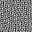
\includegraphics[width=\textwidth]{HomeWork_1/5/images/recon_p1_OMP_k=50_m=600.png}
        \caption{Reconstructed for m=600}
    \end{minipage}
    \hspace{0.5cm}
    \begin{minipage}{0.1\textwidth}
        \centering
        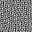
\includegraphics[width=\textwidth]{HomeWork_1/5/images/recon_p1_OMP_k=50_m=700.png}
        \caption{Reconstructed for m=700}
    \end{minipage}
    \hspace{0.5cm}
    \begin{minipage}{0.1\textwidth}
        \centering
        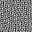
\includegraphics[width=\textwidth]{HomeWork_1/5/images/recon_p1_OMP_k=50_m=800.png}
        \caption{\small Reconstructed for m=800}
    \end{minipage}
    \hspace{0.5cm}
    \begin{minipage}{0.1\textwidth}
        \centering
        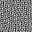
\includegraphics[width=\textwidth]{HomeWork_1/5/images/recon_p1_OMP_k=50_m=900.png}
        \caption{Reconstructed for m=900}
    \end{minipage}
    \hspace{0.5cm}
    \begin{minipage}{0.1\textwidth}
        \centering
        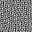
\includegraphics[width=\textwidth]{HomeWork_1/5/images/recon_p1_OMP_k=50_m=1000.png}
        \caption{Reconstructed for m=1000}
    \end{minipage}
\end{figure}

\begin{figure}[h!]
        \centering
        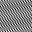
\includegraphics[width=0.25\textwidth]{HomeWork_1/5/images/orig_OMP_k=5.png}
        \caption{Original Image for k=200}
\end{figure}

\begin{figure}[h!]
    \centering
    \begin{minipage}{0.1\textwidth}
        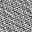
\includegraphics[width=\textwidth]{HomeWork_1/5/images/recon_p1_OMP_k=200_m=100.png}
        \caption{Reconstructed for m=100}
    \end{minipage}
    \hspace{0.5cm}
    \begin{minipage}{0.1\textwidth}
        \centering
        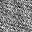
\includegraphics[width=\textwidth]{HomeWork_1/5/images/recon_p1_OMP_k=200_m=200.png}
        \caption{Reconstructed for m=200}
    \end{minipage}
    \hspace{0.5cm}
    \begin{minipage}{0.1\textwidth}
        \centering
        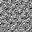
\includegraphics[width=\textwidth]{HomeWork_1/5/images/recon_p1_OMP_k=200_m=300.png}
        \caption{Reconstructed for m=300}
    \end{minipage}
    \hspace{0.5cm}
    \begin{minipage}{0.1\textwidth}
        \centering
        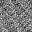
\includegraphics[width=\textwidth]{HomeWork_1/5/images/recon_p1_OMP_k=200_m=400.png}
        \caption{Reconstructed for m=400}
    \end{minipage}
    \hspace{0.5cm}
    \begin{minipage}{0.1\textwidth}
        \centering
        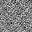
\includegraphics[width=\textwidth]{HomeWork_1/5/images/recon_p1_OMP_k=200_m=500.png}
        \caption{Reconstructed for m=500}
    \end{minipage}

    \vspace{1cm} % Add space between rows

    \begin{minipage}{0.1\textwidth}
        \centering
        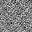
\includegraphics[width=\textwidth]{HomeWork_1/5/images/recon_p1_OMP_k=200_m=600.png}
        \caption{Reconstructed for m=600}
    \end{minipage}
    \hspace{0.5cm}
    \begin{minipage}{0.1\textwidth}
        \centering
        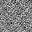
\includegraphics[width=\textwidth]{HomeWork_1/5/images/recon_p1_OMP_k=200_m=700.png}
        \caption{Reconstructed for m=700}
    \end{minipage}
    \hspace{0.5cm}
    \begin{minipage}{0.1\textwidth}
        \centering
        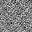
\includegraphics[width=\textwidth]{HomeWork_1/5/images/recon_p1_OMP_k=200_m=800.png}
        \caption{\small Reconstructed for m=800}
    \end{minipage}
    \hspace{0.5cm}
    \begin{minipage}{0.1\textwidth}
        \centering
        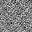
\includegraphics[width=\textwidth]{HomeWork_1/5/images/recon_p1_OMP_k=200_m=900.png}
        \caption{Reconstructed for m=900}
    \end{minipage}
    \hspace{0.5cm}
    \begin{minipage}{0.1\textwidth}
        \centering
        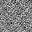
\includegraphics[width=\textwidth]{HomeWork_1/5/images/recon_p1_OMP_k=200_m=1000.png}
        \caption{Reconstructed for m=1000}
    \end{minipage}
\end{figure}

\begin{figure}[h!]
    \centering
    \begin{minipage}{0.1\textwidth}
        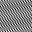
\includegraphics[width=\textwidth]{HomeWork_1/5/images/orig_OMP_k=5.png}
        \caption{Qriginal k=5}
    \end{minipage}
    \hspace{0.5cm}
    \begin{minipage}{0.1\textwidth}
        \centering
        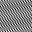
\includegraphics[width=\textwidth]{HomeWork_1/5/images/recon_p1_OMP_k=5_m=500.png}
        \caption{Reconstructed for m=500}
    \end{minipage}
    \hspace{0.5cm}
    \begin{minipage}{0.1\textwidth}
        \centering
        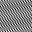
\includegraphics[width=\textwidth]{HomeWork_1/5/images/recon_p1_OMP_k=5_m=700.png}
        \caption{Reconstructed for m=700}
    \end{minipage}
\end{figure}

\begin{figure}[h!]
    \centering
    \begin{minipage}{0.1\textwidth}
        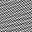
\includegraphics[width=\textwidth]{HomeWork_1/5/images/orig_OMP_k=10.png}
        \caption{Original k=10}
    \end{minipage}
    \hspace{0.5cm}
    \begin{minipage}{0.1\textwidth}
        \centering
        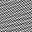
\includegraphics[width=\textwidth]{HomeWork_1/5/images/recon_p2_OMP_k=10_m=500.png}
        \caption{Reconstructed for m=500}
    \end{minipage}
    \hspace{0.5cm}
    \begin{minipage}{0.1\textwidth}
        \centering
        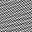
\includegraphics[width=\textwidth]{HomeWork_1/5/images/recon_p2_OMP_k=10_m=700.png}
        \caption{Reconstructed for m=700}
    \end{minipage}
\end{figure}

\begin{figure}[h!]
    \centering
    \begin{minipage}{0.1\textwidth}
        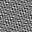
\includegraphics[width=\textwidth]{HomeWork_1/5/images/orig_OMP_k=20.png}
        \caption{Original k=20}
    \end{minipage}
    \hspace{0.5cm}
    \begin{minipage}{0.1\textwidth}
        \centering
        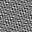
\includegraphics[width=\textwidth]{HomeWork_1/5/images/recon_p2_OMP_k=20_m=500.png}
        \caption{Reconstructed for m=500}
    \end{minipage}
    \hspace{0.5cm}
    \begin{minipage}{0.1\textwidth}
        \centering
        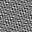
\includegraphics[width=\textwidth]{HomeWork_1/5/images/recon_p2_OMP_k=20_m=500.png}
        \caption{Reconstructed for m=700}
    \end{minipage}
\end{figure}

\begin{figure}[h!]
    \centering
    \begin{minipage}{0.1\textwidth}
        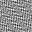
\includegraphics[width=\textwidth]{HomeWork_1/5/images/orig_OMP_k=30.png}
        \caption{original k=30}
    \end{minipage}
    \hspace{0.5cm}
    \begin{minipage}{0.1\textwidth}
        \centering
        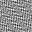
\includegraphics[width=\textwidth]{HomeWork_1/5/images/recon_p2_OMP_k=30_m=500.png}
        \caption{Reconstructed for m=500}
    \end{minipage}
    \hspace{0.5cm}
    \begin{minipage}{0.1\textwidth}
        \centering
        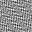
\includegraphics[width=\textwidth]{HomeWork_1/5/images/recon_p2_OMP_k=30_m=700.png}
        \caption{Reconstructed for m=700}
    \end{minipage}
\end{figure}

\begin{figure}[h!]
    \centering
    \begin{minipage}{0.1\textwidth}
        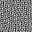
\includegraphics[width=\textwidth]{HomeWork_1/5/images/orig_OMP_k=50.png}
        \caption{Original k=50}
    \end{minipage}
    \hspace{0.5cm}
    \begin{minipage}{0.1\textwidth}
        \centering
        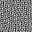
\includegraphics[width=\textwidth]{HomeWork_1/5/images/recon_p2_OMP_k=50_m=500.png}
        \caption{Reconstructed for m=500}
    \end{minipage}
    \hspace{0.5cm}
    \begin{minipage}{0.1\textwidth}
        \centering
        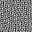
\includegraphics[width=\textwidth]{HomeWork_1/5/images/recon_p2_OMP_k=50_m=700.png}
        \caption{Reconstructed for m=700}
    \end{minipage}
\end{figure}

\begin{figure}[h!]
    \centering
    \begin{minipage}{0.1\textwidth}
        \includegraphics[width=\textwidth]{HomeWork_1/5/images/orig_OMP_k=100.png}
        \caption{Qriginal k=100}
    \end{minipage}
    \hspace{0.5cm}
    \begin{minipage}{0.1\textwidth}
        \centering
        \includegraphics[width=\textwidth]{HomeWork_1/5/images/recon_p2_OMP_k=100_m=500.png}
        \caption{Reconstructed for m=500}
    \end{minipage}
    \hspace{0.5cm}
    \begin{minipage}{0.1\textwidth}
        \centering
        \includegraphics[width=\textwidth]{HomeWork_1/5/images/recon_p2_OMP_k=100_m=700.png}
        \caption{Reconstructed for m=700}
    \end{minipage}
\end{figure}

\begin{figure}[h!]
    \centering
    \begin{minipage}{0.1\textwidth}
        \includegraphics[width=\textwidth]{HomeWork_1/5/images/orig_OMP_k=150.png}
        \caption{Qriginal k=150}
    \end{minipage}
    \hspace{0.5cm}
    \begin{minipage}{0.1\textwidth}
        \centering
        \includegraphics[width=\textwidth]{HomeWork_1/5/images/recon_p2_OMP_k=150_m=500.png}
        \caption{Reconstructed for m=500}
    \end{minipage}
    \hspace{0.5cm}
    \begin{minipage}{0.1\textwidth}
        \centering
        \includegraphics[width=\textwidth]{HomeWork_1/5/images/recon_p2_OMP_k=150_m=700.png}
        \caption{Reconstructed for m=700}
    \end{minipage}
\end{figure}

\begin{figure}[h!]
    \centering
    \begin{minipage}{0.1\textwidth}
        \includegraphics[width=\textwidth]{HomeWork_1/5/images/orig_OMP_k=200.png}
        \caption{Qriginal k=200}
    \end{minipage}
    \hspace{0.5cm}
    \begin{minipage}{0.1\textwidth}
        \centering
        \includegraphics[width=\textwidth]{HomeWork_1/5/images/recon_p2_OMP_k=200_m=500.png}
        \caption{Reconstructed for m=500}
    \end{minipage}
    \hspace{0.5cm}
    \begin{minipage}{0.1\textwidth}
        \centering
        \includegraphics[width=\textwidth]{HomeWork_1/5/images/recon_p2_OMP_k=200_m=700.png}
        \caption{Reconstructed for m=700}
    \end{minipage}
\end{figure}
\FloatBarrier
\subsection*{Comments on OMP}
We observe that RMSE increases for increasing k at a fixed m. Also, RMSE decreases for increasing m with a fixed k.
\FloatBarrier
\subsection*{CoSAMP}
\begin{figure}[h!]
    \centering
        \centering
        \includegraphics[width=0.5\textwidth]{HomeWork_1/5/images/CoSAMP_k.png}
        \caption{Plot for RMSE vs m for CoSAMP}
\end{figure}
\begin{figure}[h!]
        \centering
        \includegraphics[width=0.5\textwidth]{HomeWork_1/5/images/CoSAMP_m.png}
        \caption{Plot for RMSE vs k for CoSAMP}
\end{figure}
\begin{figure}[h!]
        \centering
        \includegraphics[width=0.25\textwidth]{HomeWork_1/5/images/orig_CoSAMP_k=5.png}
        \caption{Original Image for k=5}
\end{figure}

\begin{figure}[h!]
    \centering
    \begin{minipage}{0.1\textwidth}
        \includegraphics[width=\textwidth]{HomeWork_1/5/images/recon_p1_CoSAMP_k=5_m=100.png}
        \caption{Reconstructed for m=100}
    \end{minipage}
    \hspace{0.5cm}
    \begin{minipage}{0.1\textwidth}
        \centering
        \includegraphics[width=\textwidth]{HomeWork_1/5/images/recon_p1_CoSAMP_k=5_m=200.png}
        \caption{Reconstructed for m=200}
    \end{minipage}
    \hspace{0.5cm}
    \begin{minipage}{0.1\textwidth}
        \centering
        \includegraphics[width=\textwidth]{HomeWork_1/5/images/recon_p1_CoSAMP_k=5_m=300.png}
        \caption{Reconstructed for m=300}
    \end{minipage}
    \hspace{0.5cm}
    \begin{minipage}{0.1\textwidth}
        \centering
        \includegraphics[width=\textwidth]{HomeWork_1/5/images/recon_p1_CoSAMP_k=5_m=400.png}
        \caption{Reconstructed for m=400}
    \end{minipage}
    \hspace{0.5cm}
    \begin{minipage}{0.1\textwidth}
        \centering
        \includegraphics[width=\textwidth]{HomeWork_1/5/images/recon_p1_CoSAMP_k=5_m=500.png}
        \caption{Reconstructed for m=500}
    \end{minipage}

    \vspace{1cm} % Add space between rows

    \begin{minipage}{0.1\textwidth}
        \centering
        \includegraphics[width=\textwidth]{HomeWork_1/5/images/recon_p1_CoSAMP_k=5_m=600.png}
        \caption{Reconstructed for m=600}
    \end{minipage}
    \hspace{0.5cm}
    \begin{minipage}{0.1\textwidth}
        \centering
        \includegraphics[width=\textwidth]{HomeWork_1/5/images/recon_p1_CoSAMP_k=5_m=700.png}
        \caption{Reconstructed for m=700}
    \end{minipage}
    \hspace{0.5cm}
    \begin{minipage}{0.1\textwidth}
        \centering
        \includegraphics[width=\textwidth]{HomeWork_1/5/images/recon_p1_CoSAMP_k=5_m=800.png}
        \caption{\small Reconstructed for m=800}
    \end{minipage}
    \hspace{0.5cm}
    \begin{minipage}{0.1\textwidth}
        \centering
        \includegraphics[width=\textwidth]{HomeWork_1/5/images/recon_p1_CoSAMP_k=5_m=900.png}
        \caption{Reconstructed for m=900}
    \end{minipage}
    \hspace{0.5cm}
    \begin{minipage}{0.1\textwidth}
        \centering
        \includegraphics[width=\textwidth]{HomeWork_1/5/images/recon_p1_CoSAMP_k=5_m=1000.png}
        \caption{Reconstructed for m=1000}
    \end{minipage}
\end{figure}

\begin{figure}[h!]
        \centering
        \includegraphics[width=0.25\textwidth]{HomeWork_1/5/images/orig_CoSAMP_k=50.png}
        \caption{Original Image for k=50}
\end{figure}

\begin{figure}[h!]
    \centering
    \begin{minipage}{0.1\textwidth}
        \includegraphics[width=\textwidth]{HomeWork_1/5/images/recon_p1_CoSAMP_k=50_m=100.png}
        \caption{Reconstructed for m=100}
    \end{minipage}
    \hspace{0.5cm}
    \begin{minipage}{0.1\textwidth}
        \centering
        \includegraphics[width=\textwidth]{HomeWork_1/5/images/recon_p1_CoSAMP_k=50_m=200.png}
        \caption{Reconstructed for m=200}
    \end{minipage}
    \hspace{0.5cm}
    \begin{minipage}{0.1\textwidth}
        \centering
        \includegraphics[width=\textwidth]{HomeWork_1/5/images/recon_p1_CoSAMP_k=50_m=300.png}
        \caption{Reconstructed for m=300}
    \end{minipage}
    \hspace{0.5cm}
    \begin{minipage}{0.1\textwidth}
        \centering
        \includegraphics[width=\textwidth]{HomeWork_1/5/images/recon_p1_CoSAMP_k=50_m=400.png}
        \caption{Reconstructed for m=400}
    \end{minipage}
    \hspace{0.5cm}
    \begin{minipage}{0.1\textwidth}
        \centering
        \includegraphics[width=\textwidth]{HomeWork_1/5/images/recon_p1_CoSAMP_k=50_m=500.png}
        \caption{Reconstructed for m=500}
    \end{minipage}

    \vspace{1cm} % Add space between rows

    \begin{minipage}{0.1\textwidth}
        \centering
        \includegraphics[width=\textwidth]{HomeWork_1/5/images/recon_p1_CoSAMP_k=50_m=600.png}
        \caption{Reconstructed for m=600}
    \end{minipage}
    \hspace{0.5cm}
    \begin{minipage}{0.1\textwidth}
        \centering
        \includegraphics[width=\textwidth]{HomeWork_1/5/images/recon_p1_CoSAMP_k=50_m=700.png}
        \caption{Reconstructed for m=700}
    \end{minipage}
    \hspace{0.5cm}
    \begin{minipage}{0.1\textwidth}
        \centering
        \includegraphics[width=\textwidth]{HomeWork_1/5/images/recon_p1_CoSAMP_k=50_m=800.png}
        \caption{\small Reconstructed for m=800}
    \end{minipage}
    \hspace{0.5cm}
    \begin{minipage}{0.1\textwidth}
        \centering
        \includegraphics[width=\textwidth]{HomeWork_1/5/images/recon_p1_CoSAMP_k=50_m=900.png}
        \caption{Reconstructed for m=900}
    \end{minipage}
    \hspace{0.5cm}
    \begin{minipage}{0.1\textwidth}
        \centering
        \includegraphics[width=\textwidth]{HomeWork_1/5/images/recon_p1_CoSAMP_k=50_m=1000.png}
        \caption{Reconstructed for m=1000}
    \end{minipage}
\end{figure}

\begin{figure}[h!]
        \centering
        \includegraphics[width=0.25\textwidth]{HomeWork_1/5/images/orig_OMP_k=5.png}
        \caption{Original Image for k=200}
\end{figure}

\begin{figure}[h!]
    \centering
    \begin{minipage}{0.1\textwidth}
        \includegraphics[width=\textwidth]{HomeWork_1/5/images/recon_p1_OMP_k=200_m=100.png}
        \caption{Reconstructed for m=100}
    \end{minipage}
    \hspace{0.5cm}
    \begin{minipage}{0.1\textwidth}
        \centering
        \includegraphics[width=\textwidth]{HomeWork_1/5/images/recon_p1_OMP_k=200_m=200.png}
        \caption{Reconstructed for m=200}
    \end{minipage}
    \hspace{0.5cm}
    \begin{minipage}{0.1\textwidth}
        \centering
        \includegraphics[width=\textwidth]{HomeWork_1/5/images/recon_p1_OMP_k=200_m=300.png}
        \caption{Reconstructed for m=300}
    \end{minipage}
    \hspace{0.5cm}
    \begin{minipage}{0.1\textwidth}
        \centering
        \includegraphics[width=\textwidth]{HomeWork_1/5/images/recon_p1_OMP_k=200_m=400.png}
        \caption{Reconstructed for m=400}
    \end{minipage}
    \hspace{0.5cm}
    \begin{minipage}{0.1\textwidth}
        \centering
        \includegraphics[width=\textwidth]{HomeWork_1/5/images/recon_p1_OMP_k=200_m=500.png}
        \caption{Reconstructed for m=500}
    \end{minipage}

    \vspace{1cm} % Add space between rows

    \begin{minipage}{0.1\textwidth}
        \centering
        \includegraphics[width=\textwidth]{HomeWork_1/5/images/recon_p1_OMP_k=200_m=600.png}
        \caption{Reconstructed for m=600}
    \end{minipage}
    \hspace{0.5cm}
    \begin{minipage}{0.1\textwidth}
        \centering
        \includegraphics[width=\textwidth]{HomeWork_1/5/images/recon_p1_OMP_k=200_m=700.png}
        \caption{Reconstructed for m=700}
    \end{minipage}
    \hspace{0.5cm}
    \begin{minipage}{0.1\textwidth}
        \centering
        \includegraphics[width=\textwidth]{HomeWork_1/5/images/recon_p1_OMP_k=200_m=800.png}
        \caption{\small Reconstructed for m=800}
    \end{minipage}
    \hspace{0.5cm}
    \begin{minipage}{0.1\textwidth}
        \centering
        \includegraphics[width=\textwidth]{HomeWork_1/5/images/recon_p1_OMP_k=200_m=900.png}
        \caption{Reconstructed for m=900}
    \end{minipage}
    \hspace{0.5cm}
    \begin{minipage}{0.1\textwidth}
        \centering
        \includegraphics[width=\textwidth]{HomeWork_1/5/images/recon_p1_OMP_k=200_m=1000.png}
        \caption{Reconstructed for m=1000}
    \end{minipage}
\end{figure}

\begin{figure}[h!]
    \centering
    \begin{minipage}{0.1\textwidth}
        \includegraphics[width=\textwidth]{HomeWork_1/5/images/orig_CoSAMP_k=5.png}
        \caption{Qriginal k=5}
    \end{minipage}
    \hspace{0.5cm}
    \begin{minipage}{0.1\textwidth}
        \centering
        \includegraphics[width=\textwidth]{HomeWork_1/5/images/recon_p1_CoSAMP_k=5_m=500.png}
        \caption{Reconstructed for m=500}
    \end{minipage}
    \hspace{0.5cm}
    \begin{minipage}{0.1\textwidth}
        \centering
        \includegraphics[width=\textwidth]{HomeWork_1/5/images/recon_p1_CoSAMP_k=5_m=700.png}
        \caption{Reconstructed for m=700}
    \end{minipage}
\end{figure}

\begin{figure}[h!]
    \centering
    \begin{minipage}{0.1\textwidth}
        \includegraphics[width=\textwidth]{HomeWork_1/5/images/orig_CoSAMP_k=10.png}
        \caption{Original k=10}
    \end{minipage}
    \hspace{0.5cm}
    \begin{minipage}{0.1\textwidth}
        \centering
        \includegraphics[width=\textwidth]{HomeWork_1/5/images/recon_p2_CoSAMP_k=10_m=500.png}
        \caption{Reconstructed for m=500}
    \end{minipage}
    \hspace{0.5cm}
    \begin{minipage}{0.1\textwidth}
        \centering
        \includegraphics[width=\textwidth]{HomeWork_1/5/images/recon_p2_CoSAMP_k=10_m=700.png}
        \caption{Reconstructed for m=700}
    \end{minipage}
\end{figure}

\begin{figure}[h!]
    \centering
    \begin{minipage}{0.1\textwidth}
        \includegraphics[width=\textwidth]{HomeWork_1/5/images/orig_CoSAMP_k=20.png}
        \caption{Original k=20}
    \end{minipage}
    \hspace{0.5cm}
    \begin{minipage}{0.1\textwidth}
        \centering
        \includegraphics[width=\textwidth]{HomeWork_1/5/images/recon_p2_CoSAMP_k=20_m=500.png}
        \caption{Reconstructed for m=500}
    \end{minipage}
    \hspace{0.5cm}
    \begin{minipage}{0.1\textwidth}
        \centering
        \includegraphics[width=\textwidth]{HomeWork_1/5/images/recon_p2_CoSAMP_k=20_m=700.png}
        \caption{Reconstructed for m=700}
    \end{minipage}
\end{figure}

\begin{figure}[h!]
    \centering
    \begin{minipage}{0.1\textwidth}
        \includegraphics[width=\textwidth]{HomeWork_1/5/images/orig_CoSAMP_k=30.png}
        \caption{original k=30}
    \end{minipage}
    \hspace{0.5cm}
    \begin{minipage}{0.1\textwidth}
        \centering
        \includegraphics[width=\textwidth]{HomeWork_1/5/images/recon_p2_CoSAMP_k=30_m=500.png}
        \caption{Reconstructed for m=500}
    \end{minipage}
    \hspace{0.5cm}
    \begin{minipage}{0.1\textwidth}
        \centering
        \includegraphics[width=\textwidth]{HomeWork_1/5/images/recon_p2_CoSAMP_k=30_m=700.png}
        \caption{Reconstructed for m=700}
    \end{minipage}
\end{figure}

\begin{figure}[h!]
    \centering
    \begin{minipage}{0.1\textwidth}
        \includegraphics[width=\textwidth]{HomeWork_1/5/images/orig_CoSAMP_k=50.png}
        \caption{Original k=50}
    \end{minipage}
    \hspace{0.5cm}
    \begin{minipage}{0.1\textwidth}
        \centering
        \includegraphics[width=\textwidth]{HomeWork_1/5/images/recon_p2_CoSAMP_k=50_m=500.png}
        \caption{Reconstructed for m=500}
    \end{minipage}
    \hspace{0.5cm}
    \begin{minipage}{0.1\textwidth}
        \centering
        \includegraphics[width=\textwidth]{HomeWork_1/5/images/recon_p2_CoSAMP_k=50_m=700.png}
        \caption{Reconstructed for m=700}
    \end{minipage}
\end{figure}

\begin{figure}[h!]
    \centering
    \begin{minipage}{0.1\textwidth}
        \includegraphics[width=\textwidth]{HomeWork_1/5/images/orig_CoSAMP_k=100.png}
        \caption{Qriginal k=100}
    \end{minipage}
    \hspace{0.5cm}
    \begin{minipage}{0.1\textwidth}
        \centering
        \includegraphics[width=\textwidth]{HomeWork_1/5/images/recon_p2_CoSAMP_k=100_m=500.png}
        \caption{Reconstructed for m=500}
    \end{minipage}
    \hspace{0.5cm}
    \begin{minipage}{0.1\textwidth}
        \centering
        \includegraphics[width=\textwidth]{HomeWork_1/5/images/recon_p2_CoSAMP_k=100_m=700.png}
        \caption{Reconstructed for m=700}
    \end{minipage}
\end{figure}

\begin{figure}[h!]
    \centering
    \begin{minipage}{0.1\textwidth}
        \includegraphics[width=\textwidth]{HomeWork_1/5/images/orig_CoSAMP_k=150.png}
        \caption{Qriginal k=150}
    \end{minipage}
    \hspace{0.5cm}
    \begin{minipage}{0.1\textwidth}
        \centering
        \includegraphics[width=\textwidth]{HomeWork_1/5/images/recon_p2_CoSAMP_k=150_m=500.png}
        \caption{Reconstructed for m=500}
    \end{minipage}
    \hspace{0.5cm}
    \begin{minipage}{0.1\textwidth}
        \centering
        \includegraphics[width=\textwidth]{HomeWork_1/5/images/recon_p2_CoSAMP_k=150_m=700.png}
        \caption{Reconstructed for m=700}
    \end{minipage}
\end{figure}

\begin{figure}[h!]
    \centering
    \begin{minipage}{0.1\textwidth}
        \includegraphics[width=\textwidth]{HomeWork_1/5/images/orig_CoSAMP_k=200.png}
        \caption{Qriginal k=200}
    \end{minipage}
    \hspace{0.5cm}
    \begin{minipage}{0.1\textwidth}
        \centering
        \includegraphics[width=\textwidth]{HomeWork_1/5/images/recon_p2_CoSAMP_k=200_m=500.png}
        \caption{Reconstructed for m=500}
    \end{minipage}
    \hspace{0.5cm}
    \begin{minipage}{0.1\textwidth}
        \centering
        \includegraphics[width=\textwidth]{HomeWork_1/5/images/recon_p2_CoSAMP_k=200_m=700.png}
        \caption{Reconstructed for m=700}
    \end{minipage}
\end{figure}
\FloatBarrier
\subsection*{Comments on CoSAMP}
Similar to OMP, we observe that RMSE increases for increasing k at a fixed m. Also, RMSE decreases for increasing m with a fixed k.
However, there is a sudden steep increase in RMSE for m=500,k=200 in case of CoSAMP. This maybe due to the fact that CoSAMP requires more measurements(that is, more m) than OMP. In all other cases, the RMSE is of the order of $10^{-16}$.

\end{document}